% ======================================================================
% Paper B draft -- dynamic and quasi-static hysteresis of inertial dipolar
% rotor arrays. Sections I-V drafted from Report V61 (22/10/2026); Sections
% VI (return-point memory) and VII (discussion) wait for the Phase-3 stress
% test. Outline and open items: docs/ARTIGO_B_ROTEIRO.md.
% Compile from docs/paper_B/:  pdflatex paper_B.tex (twice)
% ======================================================================
\documentclass[pre,twocolumn,superscriptaddress,showpacs,floatfix]{revtex4-2}

\usepackage[utf8]{inputenc}
\usepackage[T1]{fontenc}
\usepackage{amsmath,amssymb}
\usepackage{graphicx}
\usepackage{siunitx}
\usepackage{xcolor}
\usepackage[colorlinks=true,linkcolor=blue!50!black,citecolor=blue!50!black,urlcolor=blue!50!black]{hyperref}

\newcommand{\vect}[1]{\boldsymbol{#1}}
\newcommand{\todo}[1]{\textcolor{red!70!black}{\textbf{[#1]}}}
\newcommand{\Bref}{B_{\rm ref}}
\newcommand{\Blat}{B_{\rm lat}}

\begin{document}

\title{Inertia selects reversal paths in the hysteresis of dipolar rotor arrays}
% Alternative titles: docs/ARTIGO_B_ROTEIRO.md, section 1. The final title
% depends on the outcome of the return-point-memory stress test.

\author{J. P. Sinnecker}
\affiliation{Centro Brasileiro de Pesquisas F\'isicas, Rio de Janeiro, Brazil}

\date{\today}

\begin{abstract}
Arrays of macroscopic compass needles are rigid rotors coupled by the long-range dipolar interaction, with genuine moment of inertia and damping. We ask how inertia, summarized by an intrinsic quality factor $Q_0$, enters their hysteresis in square, triangular and honeycomb lattices. Separating rate and inertia requires a protocol-independent $Q_0$, a dimensionless sweep rate $r$, and direct access to the quasi-static limit, which we obtain with an event-driven protocol that relaxes the array to rest after every field step and rejects zero-torque saddle points. At finite rate (690 loops, up to $64\times64$ needles), overdamped loops ($Q_0\lesssim1$) collapse when $r$ is measured in viscous relaxation times, and underdamped arrays have loops 20--50\,\% narrower than overdamped ones. In the quasi-static limit (120 loops), arrays up to $16\times16$ have the same loop for all $Q_0$, and $Q_0=1$ coincides with the gradient flow everywhere. In $24\times24$ and $32\times32$ arrays, underdamped dynamics narrows the quasi-static loop by 9--21\,\% in five of six geometry/size combinations, through avalanches whose outcome differs from the gradient flow. \todo{Return-point memory: result of the stress test.}
\end{abstract}

\maketitle

% ======================================================================
\section{Introduction}
\label{sec:intro}
% ======================================================================

Arrays of interacting magnetic dipoles are a classic model system for collective magnetism: frustration, domains, hysteresis and avalanche-like reversal arise from the long-range, anisotropic dipolar coupling alone. Macroscopic realizations with compass needles have been used to study dipolar ordering and its thermodynamics~\cite{olive1998} and the dependence of magnetization processes on the number and arrangement of the needles~\cite{novak2004}. At the nanoscale, artificial spin ice has made frustrated dipolar arrays a large field~\cite{nisoli2013,skjaervoe2020}, including field-protocol-controlled dynamics~\cite{jensen2024}, reversal mediated by effective magnetic charges~\cite{mellado2010}, relaxation pathways~\cite{menniti2025} and memory~\cite{taniguchi2025}.

A compass needle, however, is not a nanoisland. Nanomagnets follow gyromagnetic (Landau--Lifshitz--Gilbert) dynamics and switch over shape-anisotropy barriers; a needle is a mechanical rotor with true moment of inertia, viscous (and, in reality, dry) friction and no intrinsic barrier. Artificial spin ice is therefore motivation only, and no equivalence is implied. What the macroscopic system offers instead is a dipolar lattice in which inertia is a genuine, tunable parameter.

Rotatable magnets with explicit inertia and dissipation have been built and modelled before. A planar lattice of magnetic rotors relaxes into a spin-ice-like state over several time scales, and it was argued that microscopic models cannot capture these inertial effects~\cite{mellado2012}. Chains of dipolar rotors have been used to design hysteresis, the rotor time scale bounding the sweep rate below which the loop becomes rate independent~\cite{concha2017}. Separately, the dependence of the loop area on sweep rate, dynamic hysteresis, is a classic problem with scaling forms $A-A_0\propto R^\beta$~\cite{rao1990}.

These threads leave a question open: in a long-range dipolar lattice, how much of the loop is set by the energy landscape (the quasi-static loop $A_0$), how much is a rate effect ($A-A_0$), and where does inertia enter each part? Answering it requires three ingredients that are easy to get wrong: a definition of the damping strength that does not depend on the protocol, a sweep rate measured in the system's own relaxation time, and direct access to the quasi-static limit, which is out of reach by slow sweeping in large arrays. We supply all three, validate them with automated physics tests, and apply them to square, triangular and honeycomb arrays of up to $64\times64$ needles.

Two results stand out. At finite rate, inertia is a strong control parameter: overdamped loops collapse onto a single curve when the rate is measured in viscous units, and underdamped loops are much narrower. In the quasi-static limit, inertia does not modify the loop smoothly; it acts through discrete events in which the overshoot of the rotors carries an avalanche into a different basin than the gradient flow would. These events are absent up to $16\times16$ needles and narrow the loop by up to 21\,\% at $32\times32$. \todo{One sentence on return-point memory.}

Section~\ref{sec:model} defines the model and its scales, Sec.~\ref{sec:methods} the numerical methods, including the event-driven quasi-static protocol and its saddle check. Sections~\ref{sec:dynamic} and~\ref{sec:qs} report dynamic and quasi-static hysteresis. \todo{Sections VI--VII: memory and discussion.}

% ======================================================================
\section{Model and scales}
\label{sec:model}
% ======================================================================

\paragraph{Needles and lattices.} Each needle is a flat diamond-shaped steel lamina with a central pivot. In the model it is a rigid planar rotor at a fixed site $\vect r_i$, with one angle $\theta_i$ and moment $\vect m_i=m(\cos\theta_i,\sin\theta_i,0)$. The blade sets only $m=M_s\,t\,LW/2$ and $I=m_{\rm blade}(L^2+W^2)/24$, with length $L=\SI{10}{mm}$, width $W=\SI{3}{mm}$, thickness $t$, $M_s=\SI{1.59e6}{A/m}$ and steel density \SI{7850}{kg/m^3}. \todo{Thickness: $t=0.4$\,mm in all runs vs.\ 0.26\,mm in the prototype; dimensionless results unaffected; fix before submission.} The pivot spacing is $r_{\rm nn}=\SI{13}{mm}$ in all three lattices (Fig.~\ref{fig:lattices}): square (four nearest neighbours), triangular (six) and honeycomb (three). All arrays are finite with free boundaries, as in the physical object.

\begin{figure}[t]
\centering
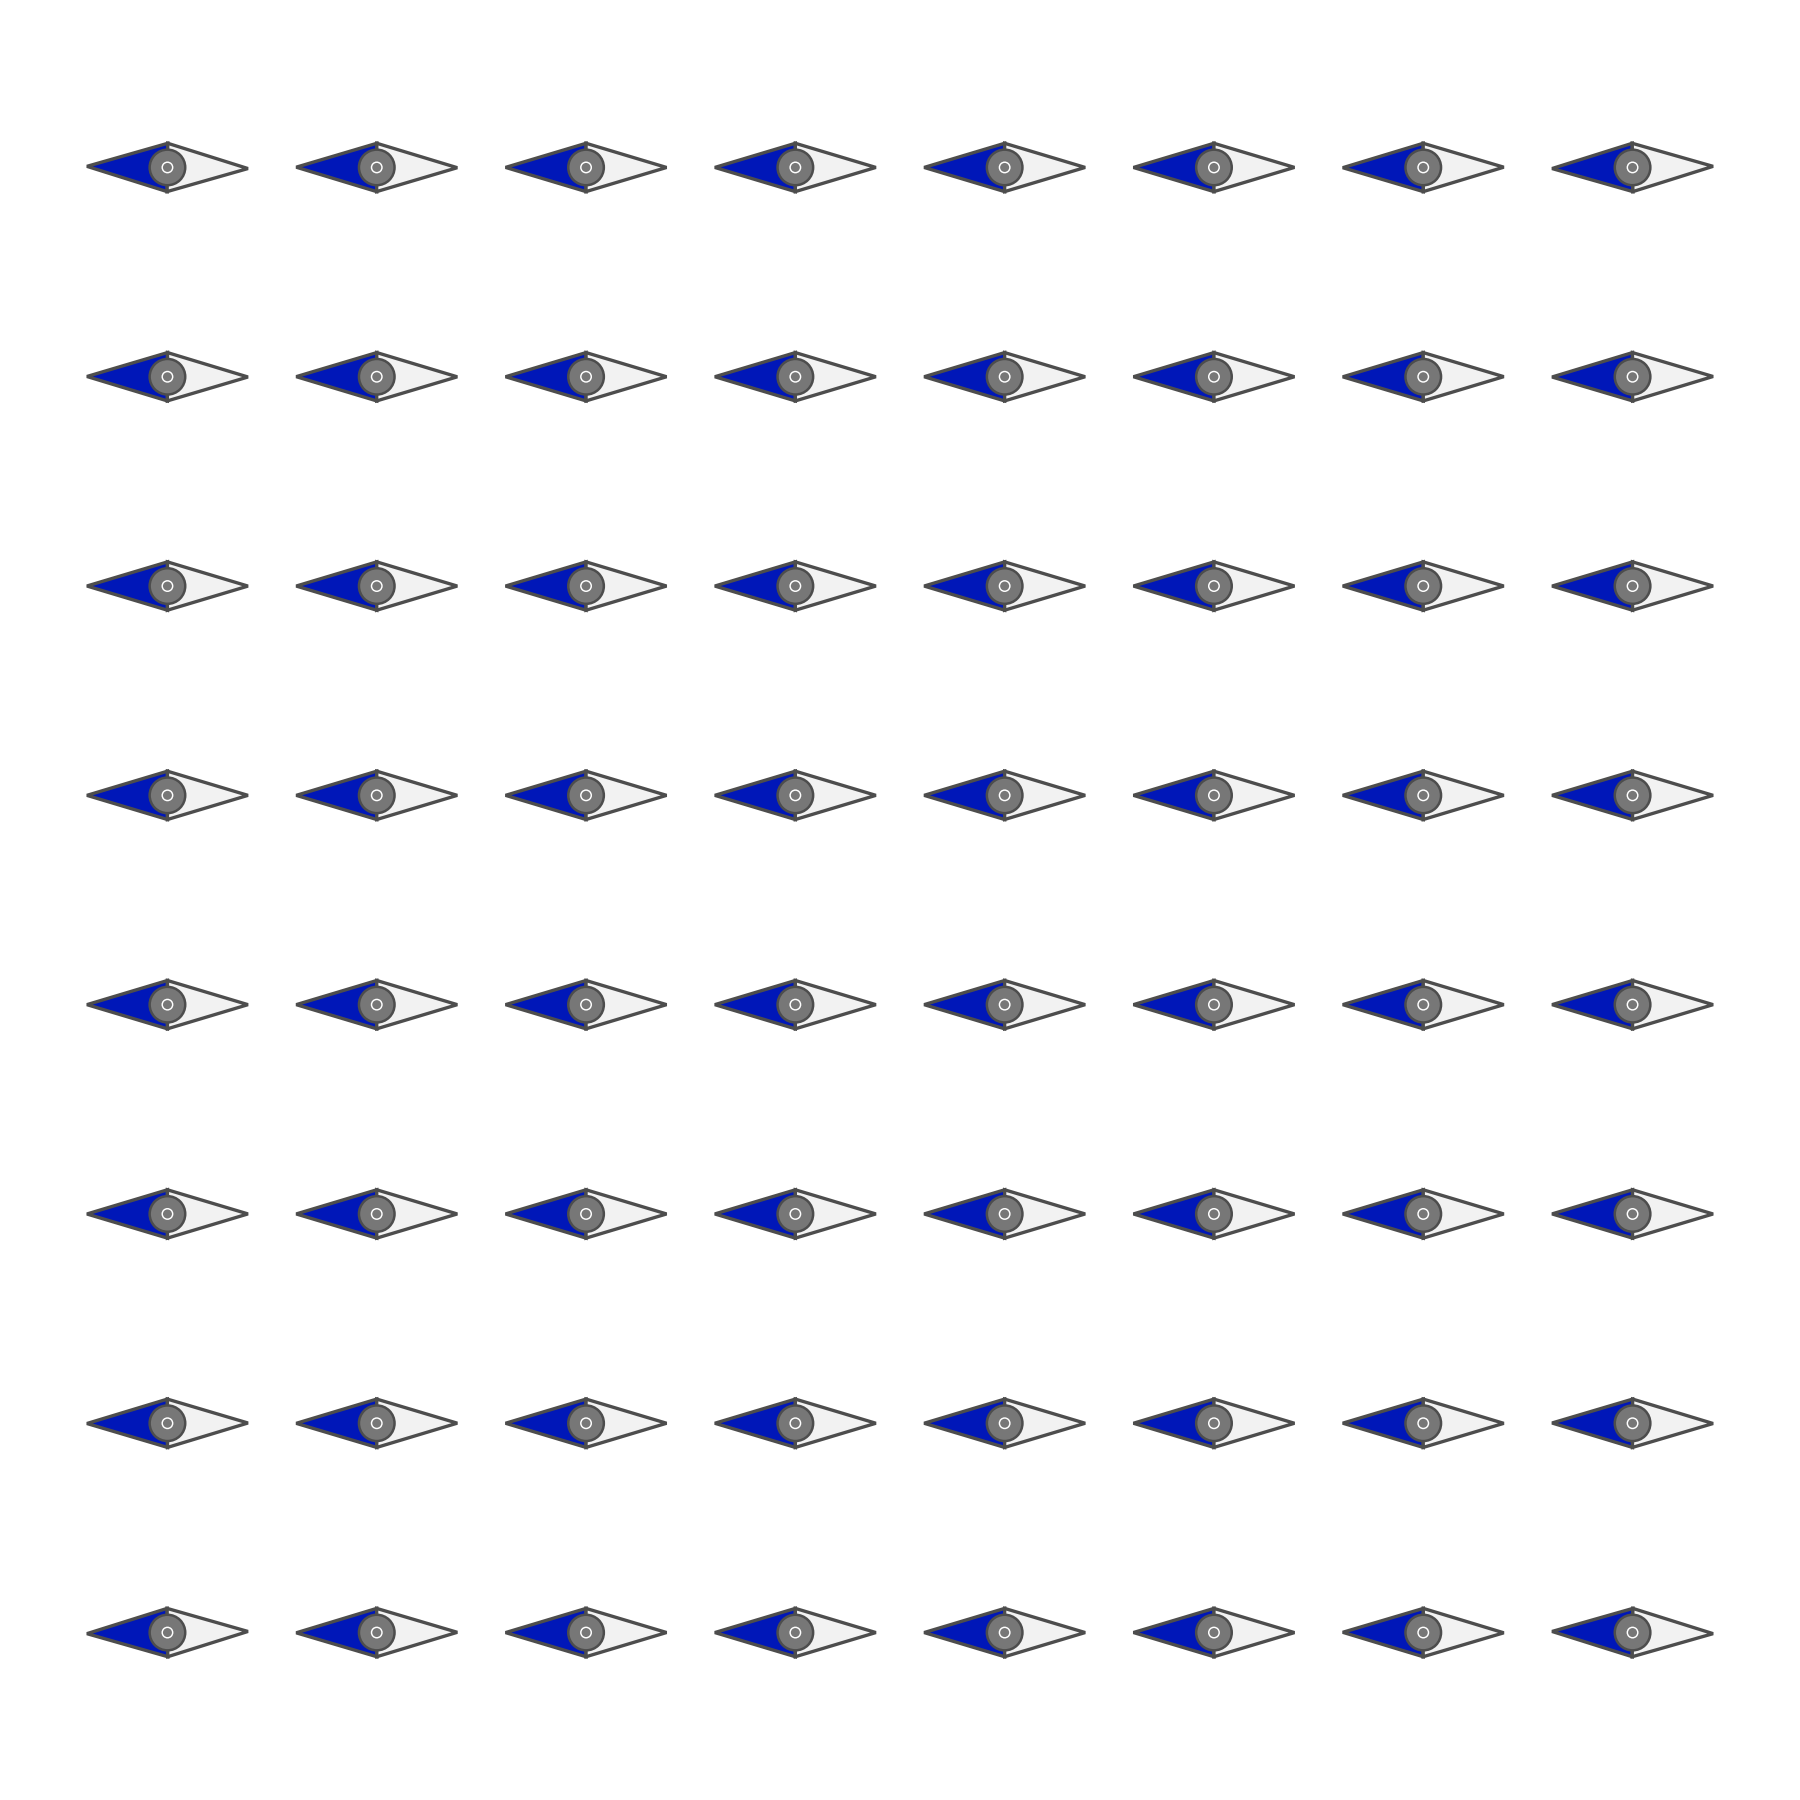
\includegraphics[width=0.32\columnwidth]{../../figs/square_default_geometry_clean_colored.png}\hfill
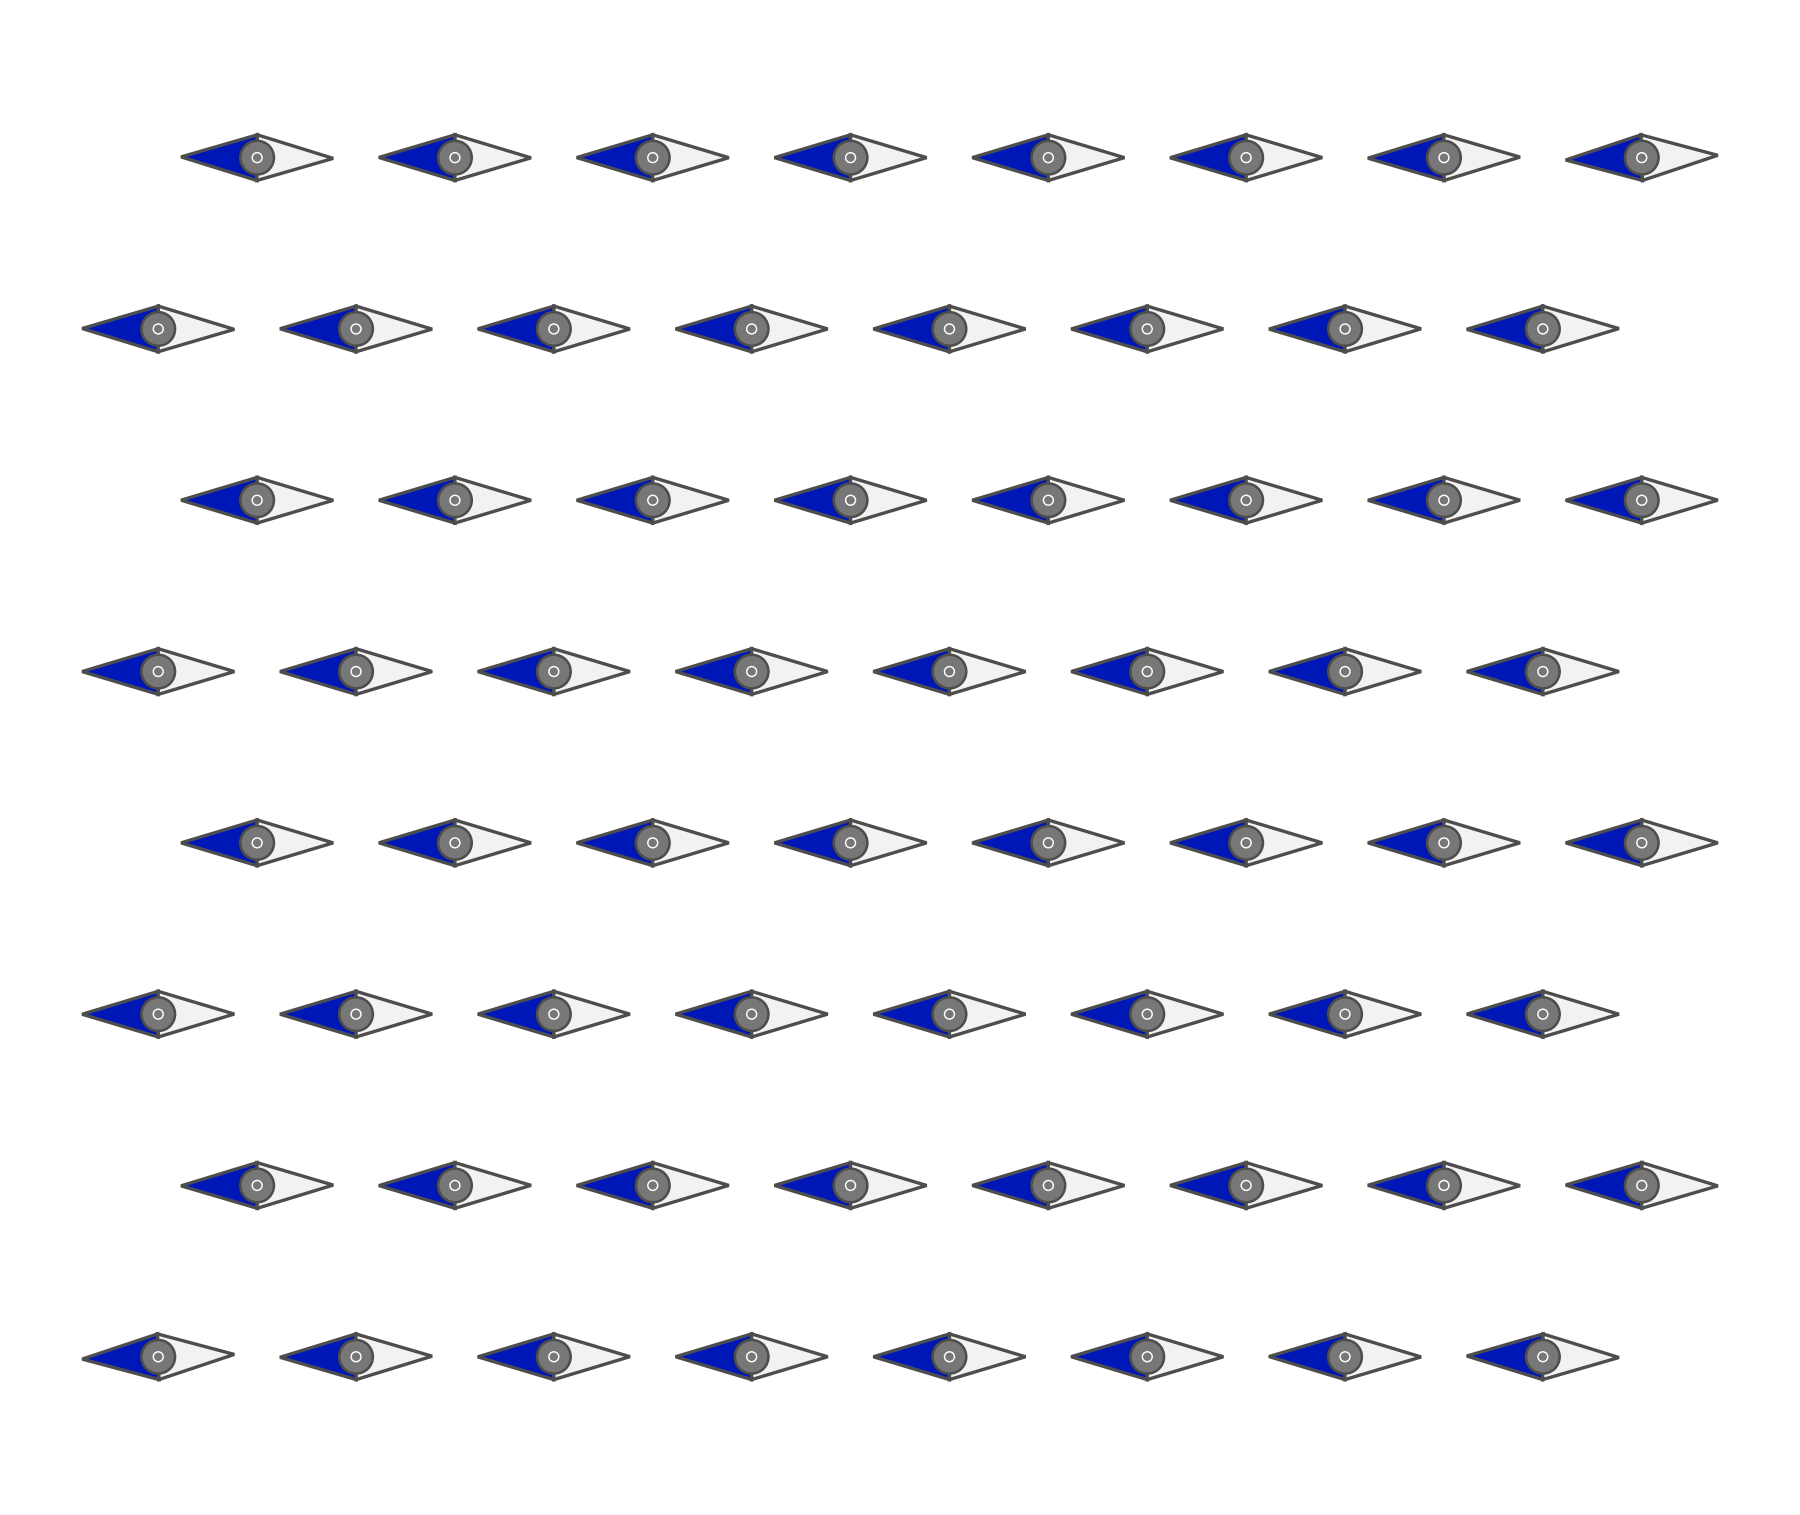
\includegraphics[width=0.32\columnwidth]{../../figs/triangular_default_geometry_clean_colored.png}\hfill
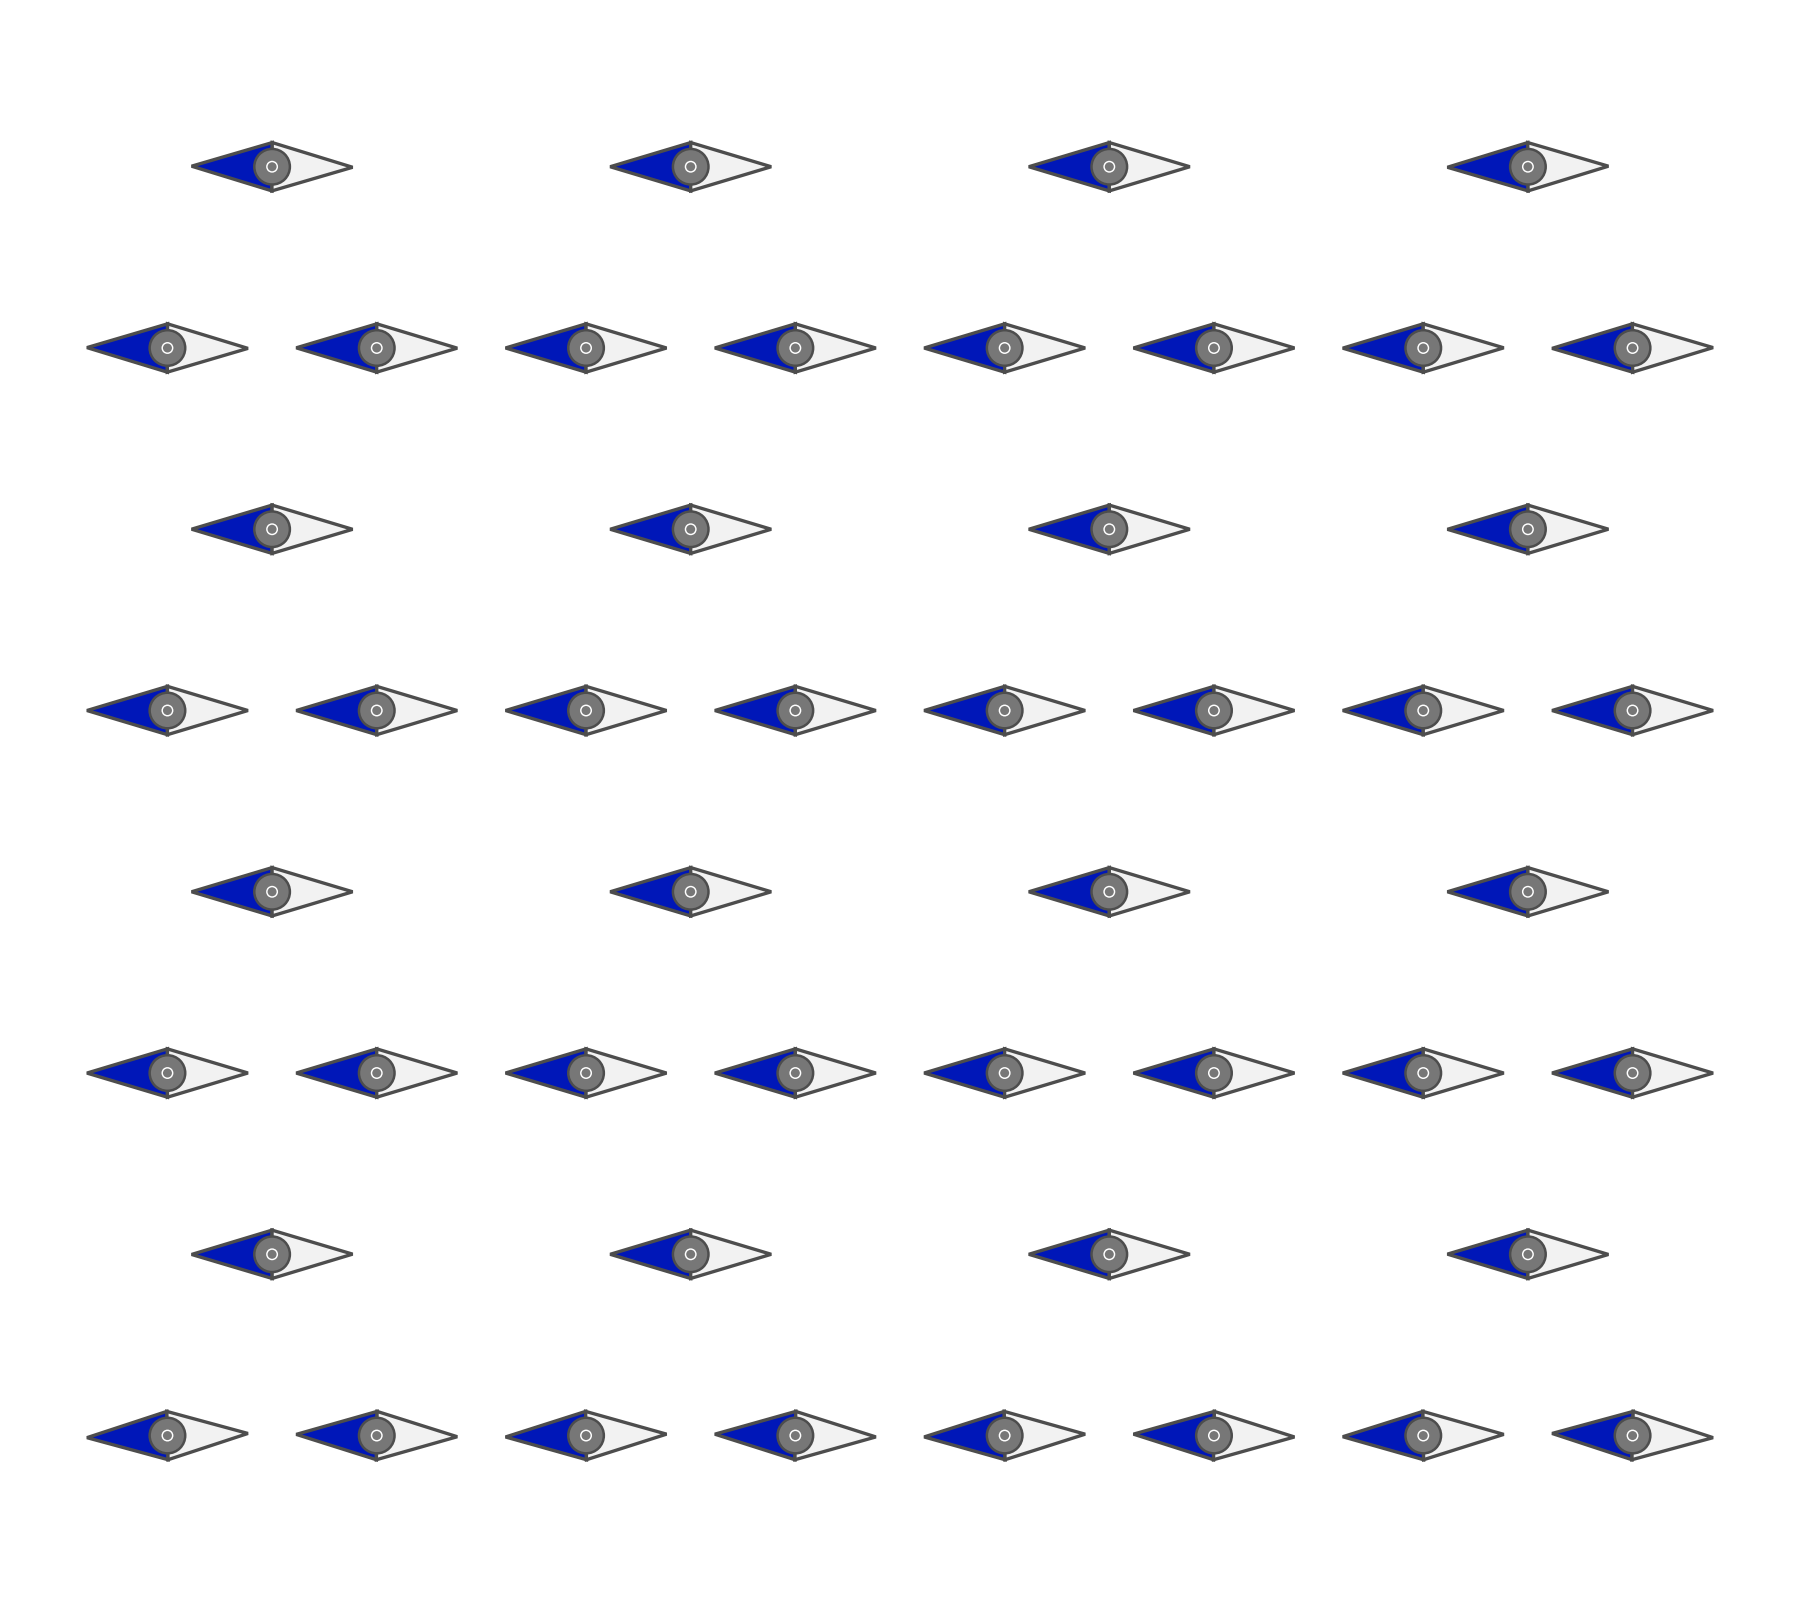
\includegraphics[width=0.32\columnwidth]{../../figs/honeycomb_default_geometry_clean_colored.png}
\caption{Square, triangular and honeycomb arrays with the same nearest-neighbour distance. \todo{Redraw as one compact panel with the needle geometry inset.}}
\label{fig:lattices}
\end{figure}

\paragraph{Dynamics.} The field at needle $i$ is the sum of the dipolar fields of all other needles and the applied field,
\begin{equation}
\vect B_i=\frac{\mu_0}{4\pi}\sum_{j\neq i}\frac{3(\vect m_j\cdot\hat{\vect r}_{ij})\hat{\vect r}_{ij}-\vect m_j}{r_{ij}^3}+\vect B_{\rm ext}(t),
\end{equation}
and each needle obeys Newton's equation for rotation with viscous damping,
\begin{equation}
I\ddot\theta_i=(\vect m_i\times\vect B_i)_z-b\,\dot\theta_i .
\label{eq:eom}
\end{equation}
The model is deterministic and athermal. The energy is $E=E_{\rm dip}+E_{\rm ext}+E_{\rm kin}$, with $E_{\rm dip}=-\tfrac12\sum_i\vect m_i\cdot\vect B_i^{\rm dip}$, $E_{\rm ext}=-\sum_i\vect m_i\cdot\vect B_{\rm ext}$ and $E_{\rm kin}=\tfrac12I\sum_i\dot\theta_i^2$. The applied field is uniform, along a lattice axis, and cycled between $\pm B_{\max}$ with $B_{\max}=4\Bref$.

\paragraph{Scales.} Fields are quoted in units of $\Bref=(\mu_0/4\pi)\,2m/r_{\rm nn}^3$, the on-axis field of a single neighbour. This is a normalization, not the field a needle feels. The intrinsic field scale of an array, $\Blat$, is the median over sites of $|\vect B_i^{\rm dip}|$ in uniform states, averaged over directions; it is $\approx2.2\Bref$ for large square arrays and smaller for small arrays, because of their edges. It defines the lattice frequency $\omega_{\rm lat}=\sqrt{m\Blat/I}$ and the intrinsic quality factor
\begin{equation}
Q_0=\frac{\omega_{\rm lat}I}{b}=\frac{\sqrt{m\Blat I}}{b},
\end{equation}
which, unlike quality factors built from the applied field, does not depend on the protocol. The relaxation time is inertial for $Q_0\ge1$ and viscous for $Q_0<1$,
\begin{equation}
\tau_{\rm relax}=\max\!\left(\frac{1}{\omega_{\rm lat}},\frac{b}{m\Blat}\right)=\frac{\max(1,1/Q_0)}{\omega_{\rm lat}},
\end{equation}
and the dimensionless sweep rate
\begin{equation}
r=\frac{dB}{dt}\,\frac{\tau_{\rm relax}}{\Bref}
\end{equation}
is the field change, in units of $\Bref$, during one relaxation time. The quasi-static limit is $r\to0$.

% ======================================================================
\section{Numerical methods}
\label{sec:methods}
% ======================================================================

\paragraph{Integration.} The dipolar interaction is precomputed as a dense $K\times K$ tensor over all pairs of the finite array, so that the fields are a matrix--vector product. Equation~\eqref{eq:eom} is integrated with velocity Verlet, with the damping treated implicitly,
\begin{equation}
\omega_i^{n+1}=\frac{\omega_i^n\left(1-\frac{b\Delta t}{2I}\right)+\frac{\Delta t}{2I}\left(\tau_i^n+\tau_i^{n+1}\right)}{1+\frac{b\Delta t}{2I}},
\end{equation}
which is symplectic at $b=0$ and stable for any $b$. The time step is $\Delta t=0.025\,T_{\rm loc}$, with $T_{\rm loc}=2\pi/\sqrt{mB_{\rm loc}/I}$ and $B_{\rm loc}$ a bound on the field any needle can feel in any configuration ($\approx6$--$8\Bref$), so that $\omega_{\rm loc}\Delta t\le0.157$ always.

\paragraph{Why these choices matter.} Each choice corrects a defect we found in earlier simulations of this system: a dipolar cutoff at $3.5\,r_{\rm nn}$ underestimated the interior field of a magnetized array by 15--17\,\% and removed the edge and shape fields; a time step set by the single-neighbour field gave energy errors of 1.8\,\% at $b=0$; a quality factor built from $\max(\Bref,B_{\rm ext})$ changed by $\sqrt8$ between protocols; and an uncontrolled sweep rate made the loop area scale roughly as (rate)$^{0.6}$, with an apparent dependence on damping that was a viscous lag. The corrected code is covered by automated tests: the tensor equals the direct pair sum to $10^{-12}$; the torque is minus the energy gradient; the energy drift at $b=0$ scales as $\Delta t^2$; $Q_0$ does not depend on the field amplitude; and the energy ledger below closes.

\paragraph{Energy ledger.} The cumulative field work $W=-\sum_i\int\vect m_i\cdot d\vect B_{\rm ext}$ and the dissipation $D=\int\sum_ib\,\dot\theta_i^2\,dt$ are integrated alongside the dynamics. They satisfy $\Delta E=W-D$ to $O(\Delta t^2)$, and over a closed cycle $W$ is the loop area. We quote the loop area per needle, $a=W/(Km\Bref)$, from the ledger; it agrees with $-\oint M\,dB$ to $5\times10^{-3}$.

\paragraph{Rate sweeps.} The field follows the loop $0\to+B_{\max}\to0\to-B_{\max}\to0\to+B_{\max}$ at constant $r$; the area is measured on the closed cycle that starts at the first arrival at $+B_{\max}$.

\paragraph{Event-driven quasi-static loops.} Sweeping cannot reach $r\to0$ in large arrays (Sec.~\ref{sec:dynamic}), so we take the limit directly. The field is changed in steps $\Delta B=0.005\Bref$. After each step, Eq.~\eqref{eq:eom} runs at fixed field, with the real $Q_0$, until $\max_i|\tau_i|\le10^{-5}m\Blat$ and $\max_i|\dot\theta_i|\le10^{-5}\omega_{\rm lat}$. The number of needles that reversed and the energy dissipated in that step define an avalanche. As the $Q_0\to0$ reference, the relaxation can instead follow the gradient flow $b\dot\theta_i=\tau_i$. The tolerance matters: on a $6\times6$ square array at $Q_0=0.3$, a loose criterion ($10^{-3}$, $\Delta B=0.02\Bref$) gives $a_0=0.710$, because relaxation stops early where the dynamics slows down critically near instabilities, while the criterion above gives $0.461$ (inertial) and $0.4606$ (gradient flow), and the slowest sweep ($r=3\times10^{-4}$) gives $0.473$.

\paragraph{Saddle check.} A state with zero torque and zero velocity can be a saddle of the energy. The gradient flow preserves the symmetry of the array exactly and can stay on a symmetric branch after that branch has become unstable. Each rest state is therefore perturbed by random kicks of $10^{-4}$\,rad and relaxed again before it is recorded; the kick energy is booked in the ledger. Without this check, small honeycomb arrays spent hundreds of field steps on saddles, and the gradient flow and the inertial dynamics appeared to differ by up to 43\,\% (Appendix~\ref{app:saddle}). \todo{Short sentence: field programs with arbitrary turning points (for Sec.~VI).}

% ======================================================================
\section{Dynamic hysteresis}
\label{sec:dynamic}
% ======================================================================

We ran 600 loops on three geometries, $N=6$, 10, 16, 24 and 32 ($N\times N$ needles), $Q_0=0.1$, 0.3, 1, 3 and 10, and $r$ from $10^{-1}$ to $10^{-3}$ (down to $3\times10^{-4}$ for $N\le16$), plus seed checks; 90 further loops cover $N=48$ and 64 ($Q_0=0.3$, 1, 3; $r\ge10^{-3}$) on a GPU. The damping was set per geometry and size so that $Q_0$ is exact. All runs closed the energy ledger to $1.2\times10^{-3}$ and reached $M\ge0.995$ at $B_{\max}$.

\begin{figure*}[t]
\centering
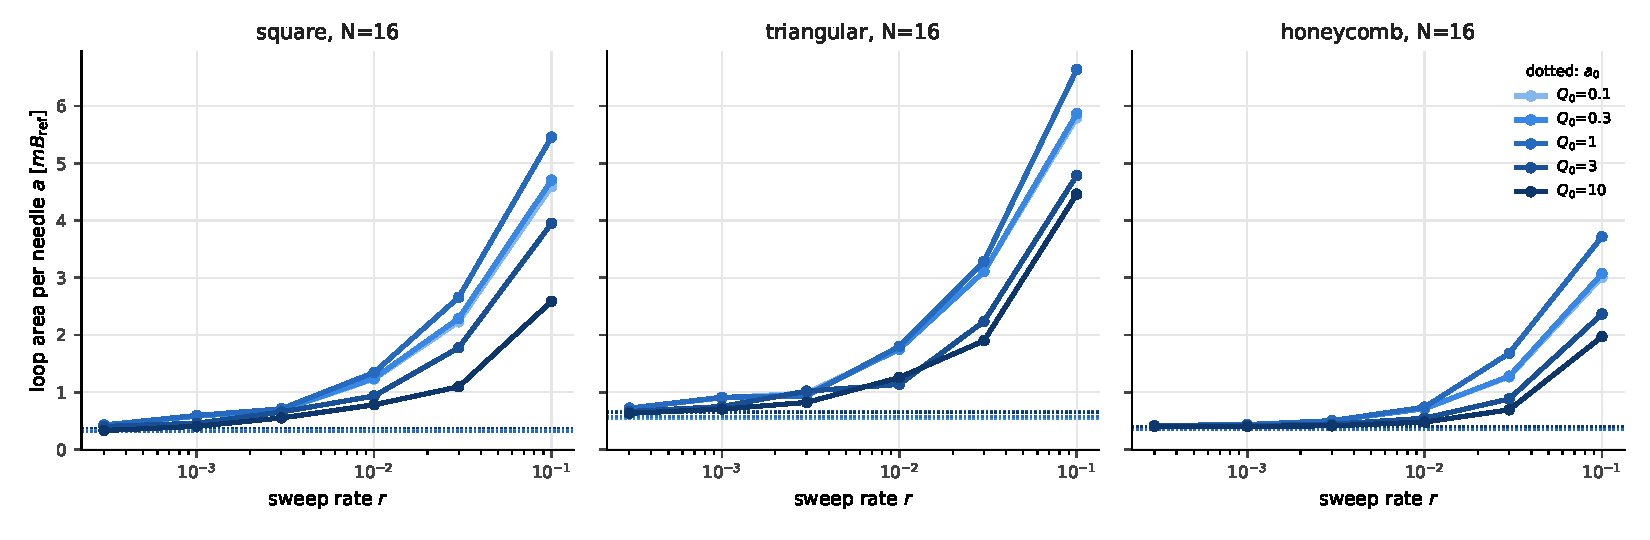
\includegraphics[width=0.8\textwidth]{../figs/fig1_area_vs_rate.pdf}
\caption{Loop area per needle $a$ (units of $m\Bref$) versus dimensionless sweep rate $r$ for $16\times16$ arrays. The curves for $Q_0=0.1$ and 0.3 (and largely $Q_0=1$) coincide: with $r$ in viscous units, overdamped dynamics is a rescaling of time. Underdamped arrays ($Q_0=3$, 10) have narrower loops at the same $r$. \todo{Remove the dotted $a_0$ fits or replace them by the quasi-static $a_0$ of Sec.~V.}}
\label{fig:area_rate}
\end{figure*}

\paragraph{Overdamped collapse.} For $Q_0=0.1$ and 0.3 the areas differ by at most 2.4\,\% over all geometries, sizes and rates (Fig.~\ref{fig:area_rate}). In the overdamped limit Eq.~\eqref{eq:eom} reduces to $b\dot\theta=\tau$, and $b$ only sets the time unit; measuring $r$ in units of $b/(m\Blat)$ removes it. Any apparent dependence on damping for $Q_0\lesssim1$ at a fixed simulation time is therefore a rate effect.

\paragraph{Inertial narrowing.} At the same $r$, raising $Q_0$ from 0.1 to 10 reduces the loop area by 22--44\,\% at $r=10^{-1}$ and by 28--54\,\% at $r=10^{-2}$, depending on geometry and size. Underdamped loops show ringing and discrete jumps (Fig.~\ref{fig:loops}).

\begin{figure}[t]
\centering
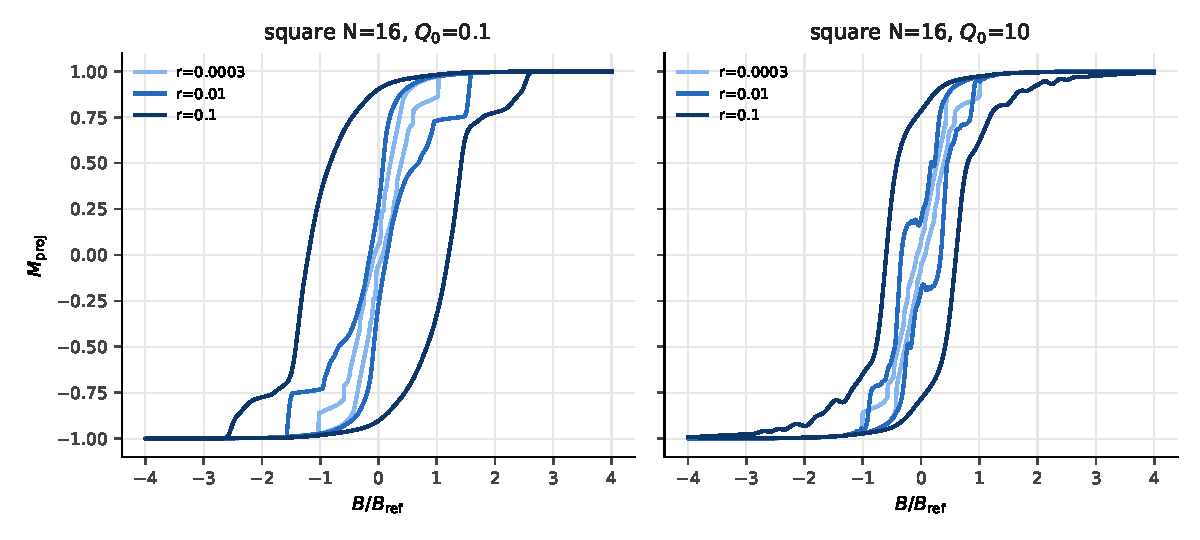
\includegraphics[width=\columnwidth]{../figs/fig4_loops.pdf}
\caption{Loops $M(B)$ of a $16\times16$ square array at three sweep rates, overdamped ($Q_0=0.1$, left) and underdamped ($Q_0=10$, right). Faster sweeps widen the loop; underdamped loops ring and jump.}
\label{fig:loops}
\end{figure}

\paragraph{The quasi-static limit is out of reach by sweeping.} For $N\ge24$ the area still changes by 40--98\,\% between $r=3\times10^{-3}$ and $10^{-3}$, and fits $a(r)=a_0+c\,r^\beta$ do not constrain $a_0$. Since the cost of a sweep grows as $1/r$, and faster still for $Q_0<1$, reaching $r\sim10^{-5}$ is prohibitive. This motivates the event-driven protocol of Sec.~\ref{sec:qs}.

\paragraph{Size and realizations.} At $r=10^{-3}$ the area levels off for $N\ge32$: for $Q_0=0.3$, square arrays give $a=0.265$, 0.238 and 0.235 at $N=32$, 48 and 64; honeycomb arrays $\approx0.42$; triangular arrays 0.73--0.69. Below $N\approx24$ the dependence is non-monotonic, reflecting edges and, for the triangular lattice, the shape of the cut. With uniform damping the saturated state erases the initial state in most conditions, but in underdamped honeycomb arrays the area varied by up to 27\,\% between initial states; Sec.~\ref{sec:qs} shows that this is a finite-rate effect.

% ======================================================================
\section{The quasi-static limit}
\label{sec:qs}
% ======================================================================

We computed 120 quasi-static loops: three geometries, $N=6$--32, four relaxation dynamics (gradient flow and $Q_0=1$, 3, 10) and two seeds, with 4000 field steps each. The ledger closed to $4\times10^{-4}$ for the inertial runs and to $8.4\times10^{-3}$ for the gradient flow, whose Euler step carries a small kinetic-energy bookkeeping term; 0.02\,\% of the field steps reached the relaxation-time cap before the tolerance, almost all in gradient-flow or $Q_0=1$ runs on large arrays, where soft modes relax slowly.

\begin{figure*}[t]
\centering
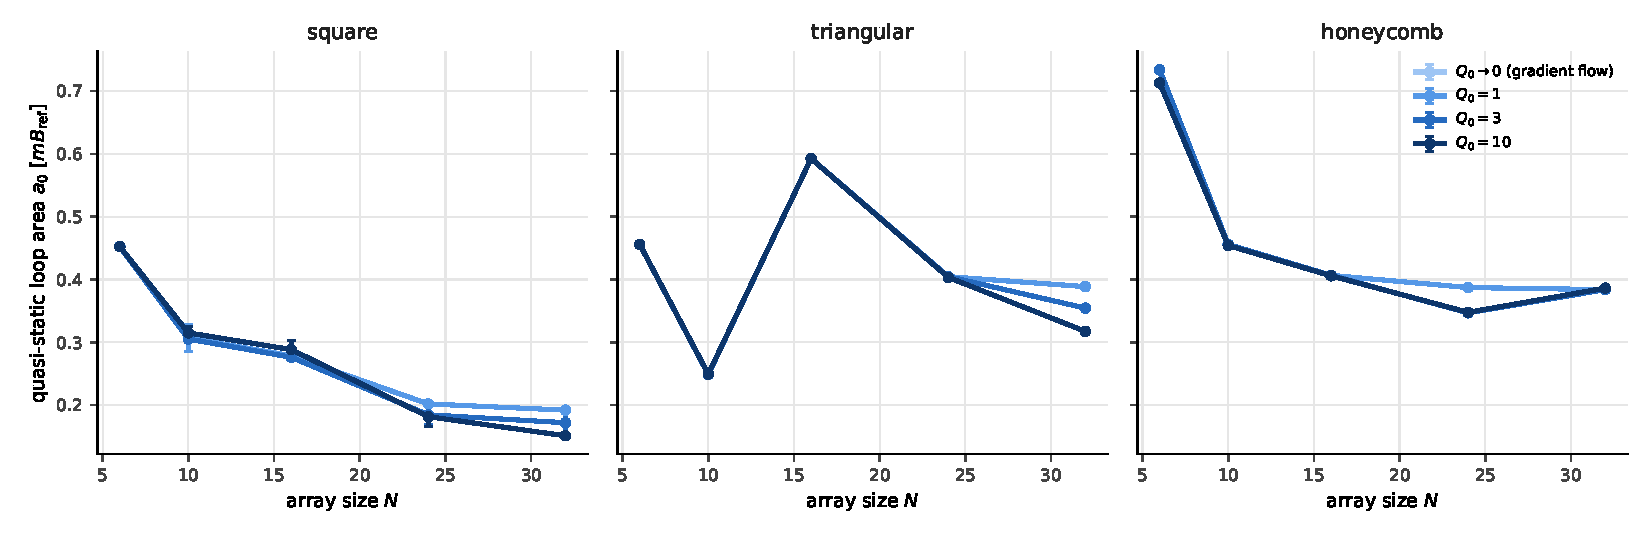
\includegraphics[width=0.8\textwidth]{../figs/figQS1_a0_vs_N.pdf}
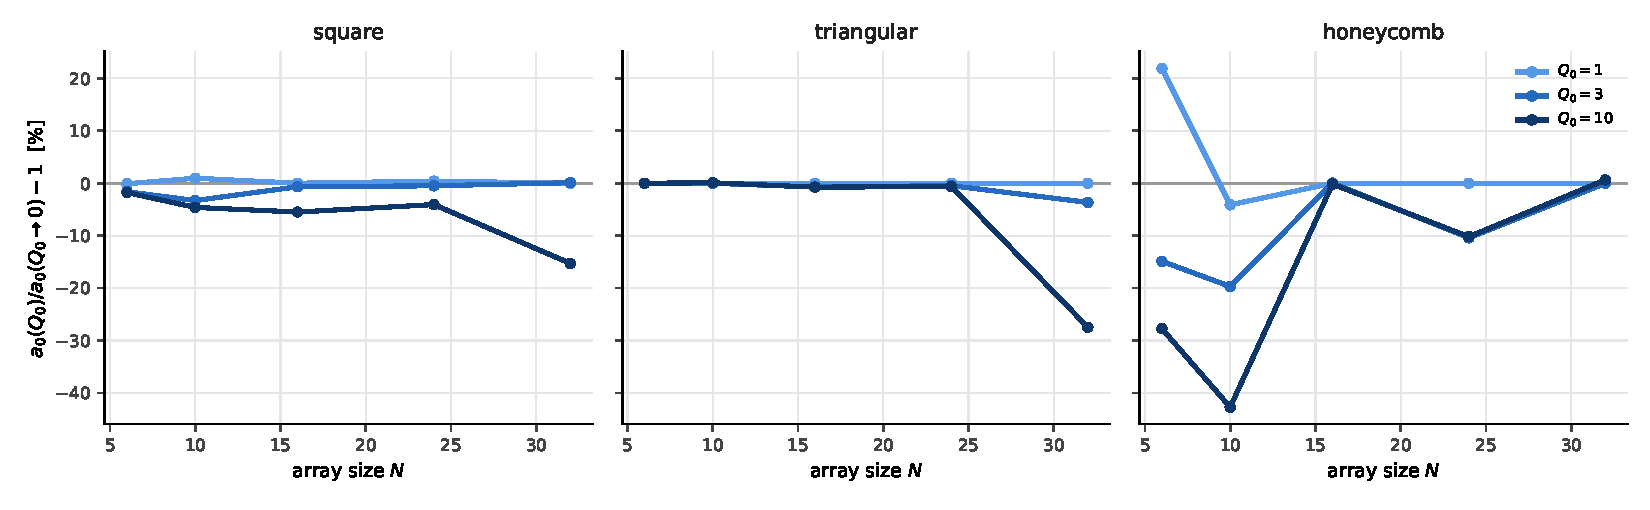
\includegraphics[width=0.8\textwidth]{../figs/figQS2_inertial_effect.pdf}
\caption{Top: quasi-static loop area $a_0$ versus array size for the four relaxation dynamics (bars: range over two seeds). Bottom: inertial effect $a_0(Q_0)/a_0(Q_0\to0)-1$. Up to $N=16$ all dynamics give the same area; at $N=24$ and 32 the underdamped loops are narrower in five of the six geometry/size combinations.}
\label{fig:qs}
\end{figure*}

\paragraph{Critical damping is already the gradient flow.} In all 15 geometry/size combinations the $Q_0=1$ loop coincides with the gradient-flow loop within $10^{-3}$. A critically damped rotor does not overshoot, so it visits the same sequence of basins.

\paragraph{Small arrays: no inertial effect.} For $N\le16$ the area changes with $Q_0$ by less than 1\,\% in triangular and honeycomb arrays, except honeycomb $6\times6$ at $Q_0=10$ ($-2.9$\,\%). In square arrays the $Q_0=10$ loop differs by $+2.7$\,\% ($10\times10$) and $+3.5$\,\% ($16\times16$), within the seed-to-seed variation of those conditions. Despite the large inertial effect at finite rate, the quasi-static loop of a small array is fixed by the energy landscape.

\paragraph{Large arrays: inertia selects narrower loops.} At $N=24$ and 32, underdamped loops are narrower than the gradient-flow loop in five of the six combinations (Fig.~\ref{fig:qs}): square $24\times24$ ($Q_0=3$: $-9$\,\%; $Q_0=10$: $-10$\,\%), square $32\times32$ ($-10$\,\%, $-21$\,\%), triangular $32\times32$ ($-9$\,\%, $-18$\,\%) and honeycomb $24\times24$ ($-10$\,\% for both). Triangular $24\times24$ and honeycomb $32\times32$ show no effect ($\le0.6$\,\%). When inertia changes the loop, it always narrows it. The coercive field and remanence change with the area; for triangular $32\times32$ at $Q_0=10$ the remanence drops from 0.22 to 0.07. These differences exceed the ledger and discretization uncertainties by two orders of magnitude.

\paragraph{Mechanism: path selection.} The pattern is that of discrete path selection. In a few large avalanches the overshoot of the rotors carries the array into a different basin than the gradient flow would, and the subsequent branch of the loop changes. In triangular $32\times32$, for example, both dynamics nucleate reversed domains in the same two corners, but the underdamped avalanche is larger and connects them, and the two loops follow different sequences of avalanches from there on. \todo{Figure: spatial map of this event, regenerated from the corrected grid.} Because the effect rests on a few events, it is not monotonic in $N$ and depends on geometry; larger arrays have more and larger avalanches, which makes such events more likely, but two sizes per geometry do not establish a trend.

\paragraph{Realizations.} In triangular and honeycomb arrays the two seeds give identical quasi-static loops (spread $\le10^{-3}$): the initial-state dependence of the underdamped sweeps is a finite-rate effect. Square arrays are different. In seven conditions the seeds differ by 7--23\,\%, for instance square $32\times32$ at $Q_0=3$ gives $a_0=0.152$ for one seed and 0.191, equal to the gradient flow, for the other. Since the seed also fixes the random kicks of the saddle check, it chooses which branch the array takes at a symmetric branch point; the square lattice, with its degenerate reversal paths, is where this matters. Two seeds only bracket this realization dependence.

\paragraph{Avalanches.} Over the closed cycle the per-step avalanche-size distributions are broad and cut off by the system size (largest events $\approx200$ needles, 20\,\% of a $32\times32$ square or triangular array) and similar for all dynamics. With these sizes we do not attempt any scaling analysis.

% ======================================================================
\section{Return-point memory}
\label{sec:rpm}
% ======================================================================
\todo{Pilot (24$\times$24, one turning point per geometry): exact return-point memory for all dynamics, with excursions that reversed up to 67\,\% of the needles. Stress test running (many turning points, nested loops, $N=6$--32); a $6\times6$ honeycomb gradient-flow check already violates memory. To be written after the stress test.}

% ======================================================================
\section{Discussion}
\label{sec:discussion}
% ======================================================================
\todo{Rate vs.\ inertia vs.\ landscape; path selection without loss of memory (if confirmed); cooperative head-to-tail coupling as a possible reason; predictions for a tabletop experiment; limitations: point dipoles (needle length 0.77 of the spacing), viscous damping only, $T=0$, free boundaries, sizes $\le32$ (quasi-static) and $\le64$ (sweeps).}

\begin{acknowledgments}
\todo{Funding (CNPq, FAPERJ, \ldots).}
\end{acknowledgments}

\appendix
\section{Saddle points in quasi-static protocols}
\label{app:saddle}
\todo{Condense the path-selection note (QS\_SELECAO\_DE\_CAMINHO): how zero-torque saddles appear (symmetric honeycomb arrays, gradient flow), how much they changed the first grid (up to 43\,\%), and why kick-and-relax removes them (areas unchanged for kicks of $10^{-4}$--$10^{-2}$\,rad).}

\begin{thebibliography}{99}
\bibitem{olive1998} E.~Olive and P.~Molho, Phys.\ Rev.\ B \textbf{58}, 9238 (1998).
\bibitem{novak2004} R.~L.~Novak and J.~P.~Sinnecker, J.\ Magn.\ Magn.\ Mater.\ \textbf{272--276}, 1557 (2004).
\bibitem{nisoli2013} C.~Nisoli, R.~Moessner, and P.~Schiffer, Rev.\ Mod.\ Phys.\ \textbf{85}, 1473 (2013).
\bibitem{skjaervoe2020} S.~H.~Skj\ae rv\o, C.~H.~Marrows, R.~L.~Stamps, and L.~J.~Heyderman, Nat.\ Rev.\ Phys.\ \textbf{2}, 13 (2020).
\bibitem{jensen2024} J.~H.~Jensen \emph{et al.}, Nat.\ Commun.\ \textbf{15}, 964 (2024).
\bibitem{mellado2010} P.~Mellado, O.~Petrova, Y.~Shen, and O.~Tchernyshyov, Phys.\ Rev.\ Lett.\ \textbf{105}, 187206 (2010).
\bibitem{menniti2025} M.~Menniti, N.~Leo, P.~Villalba-Gonz\'alez, M.~Pancaldi, and P.~Vavassori, Phys.\ Rev.\ B \textbf{112}, 134410 (2025). \todo{verify}
\bibitem{taniguchi2025} T.~Taniguchi, Sci.\ Rep.\ \textbf{15}, 9073 (2025). \todo{verify}
\bibitem{mellado2012} P.~Mellado, A.~Concha, and L.~Mahadevan, Phys.\ Rev.\ Lett.\ \textbf{109}, 257203 (2012).
\bibitem{concha2017} A.~Concha \emph{et al.}, arXiv:1710.08391 (2017). \todo{verify authors and journal version}
\bibitem{rao1990} M.~Rao, H.~R.~Krishnamurthy, and R.~Pandit, Phys.\ Rev.\ B \textbf{42}, 856 (1990).
\bibitem{sethna1993} J.~P.~Sethna, K.~Dahmen, S.~Kartha, J.~A.~Krumhansl, B.~W.~Roberts, and J.~D.~Shore, Phys.\ Rev.\ Lett.\ \textbf{70}, 3347 (1993).
\bibitem{keim2019} N.~C.~Keim, J.~D.~Paulsen, Z.~Zeravcic, S.~Sastry, and S.~R.~Nagel, Rev.\ Mod.\ Phys.\ \textbf{91}, 035002 (2019).
\end{thebibliography}

\end{document}
